\documentclass[9pt]{beamer}

%~~~~~~~~~~~~~~~~~~~~~~~~~~~~~~~~~~~~~~~~~~~~~~~~~~~~~~~~~~~~~~~~~~~~~~~~~~~~~~
% Use roboto Font (recommended)
\usepackage[sfdefault]{roboto}
\usepackage[utf8]{inputenc}
\usepackage[T1]{fontenc}
\usepackage{xeCJK}
\usepackage{amsmath,amsthm,amsfonts,amssymb,bm}
\usefonttheme[onlymath]{serif} %修改字体为数学字体
\usepackage{graphicx}%导入图片
%~~~~~~~~~~~~~~~~~~~~~~~~~~~~~~~~~~~~~~~~~~~~~~~~~~~~~~~~~~~~~~~~~~~~~~~~~~~~~~

%~~~~~~~~~~~~~~~~~~~~~~~~~~~~~~~~~~~~~~~~~~~~~~~~~~~~~~~~~~~~~~~~~~~~~~~~~~~~~~
% Define where theme files are located. ('/styles')
\usepackage{styles/fluxmacros}
\usefolder{styles}
% Use Flux theme v0.1 beta
% Available style: asphalt, blue, red, green, gray 
\usetheme[style=blue]{flux}
%~~~~~~~~~~~~~~~~~~~~~~~~~~~~~~~~~~~~~~~~~~~~~~~~~~~~~~~~~~~~~~~~~~~~~~~~~~~~~~

%~~~~~~~~~~~~~~~~~~~~~~~~~~~~~~~~~~~~~~~~~~~~~~~~~~~~~~~~~~~~~~~~~~~~~~~~~~~~~~
% Extra packages for the demo:
\usepackage{booktabs}
\usepackage{colortbl}
\usepackage{ragged2e}
\usepackage{schemabloc}
%~~~~~~~~~~~~~~~~~~~~~~~~~~~~~~~~~~~~~~~~~~~~~~~~~~~~~~~~~~~~~~~~~~~~~~~~~~~~~~

%~~~~~~~~~~~~~~~~~~~~~~~~~~~~~~~~~~~~~~~~~~~~~~~~~~~~~~~~~~~~~~~~~~~~~~~~~~~~~~
% Informations
\title{微积分习题课}
\subtitle{9月23日}
\author{徐金华}
\institute{数学科学学院,浙江大学 }
\date{\today}
\titlegraphic{assets/zju.pdf}
%~~~~~~~~~~~~~~~~~~~~~~~~~~~~~~~~~~~~~~~~~~~~~~~~~~~~~~~~~~~~~~~~~~~~~~~~~~~~~~

\begin{document}

% Generate title page
\titlepage

\begin{frame}
 \frametitle{目录}
 \tableofcontents
\end{frame}

\section{重点内容回顾}

\subsection{集合与函数}

\begin{frame}{集合}{定义}
	\justifying
 集合是具有某种特定性质,具体或抽象的对象汇成的全体\footnote{陈纪修等编著.数学分析\ 上[M].北京:高等教育出版社.2004.06:2.}\\
 
常见的表示方法有枚举法与描述法\\
\end{frame}
\begin{frame}{集合}{例子}
 	\begin{itemize}
		\item \{红,黄,蓝\}
		\item $\mathbb{N}^{+}=\{1,2,3,...,n,...\}$
		\item $\mathbb{Z}=\{0,\pm 1,\pm 2,\pm 3,...,\pm n,...\}$
		\item $\mathbb{B}=\{x:x^2=2\}$
		\item $\mathbb{Q}=\{x:x=\dfrac{q}{p},\text{其中}p \in \mathbb{N}^{+},q \in \mathbb{Z}\}$
		\item \example{$S_1=\{x:x \notin x\}$,罗素悖论、理发师悖论\footnote{杜国平.罗素悖论研究进展[J].湖北大学学报(哲学社会科学版),2012,39(5):1-6. 2012.05.001.}}
	\end{itemize}
\end{frame}

\begin{frame}{函数}{定义}
设$D$、$B$是两个非空实数集,如果存在一个对应法则$f$,使得对$D$中任何一个实数$x$,在$B$中都有唯一确定的实数$y$与$x$对应,则称对应法则$f$是$D$上的函数,记为\\
\begin{equation*}
    f:x \mapsto y \quad \text{或者} \quad f:D \xrightarrow[]{} B
\end{equation*}
 
 $y$称为$x$对应的函数值,记为\\
 \begin{equation*}
    y=f(x),\quad x \in D
\end{equation*}
 
 其中$x$叫自变量,$y$叫因变量
\end{frame}

\subsection{图像与函数图像}
\begin{frame}{图像}{}
图像是二维平面$\mathbb{R}^2$的子集,是满足某些具有特定性质的点的集合,记为\\
\begin{equation*}
    D=\{(x,y):x \text{和} y \text{满足的性质}\}
\end{equation*}
 
 例如单位圆:\\
\begin{equation*}
    O=\{(x,y):x^2+y^2=1\}
\end{equation*}
\end{frame}

\begin{frame}{函数图像}{}
函数图像只需要把$x$和$y$满足的性质换成$x$与$y$之间的函数关系
\begin{equation*}
    D=\{(x,y):\text{满足} y=f(x),x\in D\}
\end{equation*}
 
 例如正弦函数图像:\\
\begin{equation*}
    \{(x,y):y=sin(x),x \in \mathbb{R}\}
\end{equation*}
\end{frame}
\begin{frame}{函数图像}
\begin{figure}[h]
\centering
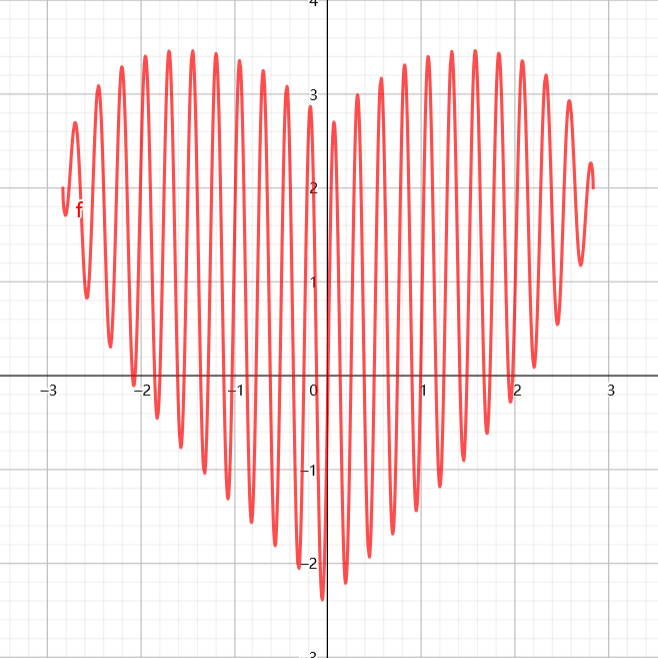
\includegraphics[width=5.5cm,height=5.5cm]{assets/heart.png}
\caption{$f(x)=x^{\frac{2}{3}}+0.9\sqrt{8-x^2}sin(25x)$}
\end{figure}
\end{frame}
%%%%%%%%%%%%%%%%%%%%%%%%%%%%%%%%%%%%%%%%%%
\subsection{反函数与反函数图像}
\begin{frame}{反函数}{定义}
设$y=f(x),x \in D$.若对$R(f)$中每一个$y$,都有唯一确定且满足$y=f(x)$的$x$与之对应,则按照此对应法则就能得到一个定义在$R(f)$上的函数,称这个函数为$f$的反函数,记作\\
\begin{equation*}
    f^{-1}:R(f) \xrightarrow[]{} D \quad \text{或} \quad x=f^{-1}(y),\ y \in R(f)
\end{equation*}
 
由于习惯上用$x$表示自变量,$y$表示因变量,所以常把上述反函数改写成\\
 \begin{equation*}
    y=f^{-1}(x),\quad x \in f(D)
\end{equation*}
\end{frame}

\subsection{函数图像的平移、拉伸与对称}
\begin{frame}{函数图像的平移、拉伸与对称}{定义}
对于给定函数$y=f(x),x \in D$,考虑一下几个函数\\
\begin{itemize}
        \item $y=f(x+a),\quad x+a\in D$,$a$为常数
        \item $y=f(x)+a$,$a$为常数
		\item $y=af(x)$,$a$为常数
		\item $y=f(ax),\quad ax\in D$,$a$为常数
		\item $y=f(-x),\quad -x\in D$
		\item $y=-f(x)$
\end{itemize}
\end{frame}
\section{课后习题}
\subsection{反函数}
\begin{frame}{19}{(4)}
求下列函数的反函数\\
\begin{equation*}
    y=\sqrt[3]{x+\sqrt{1+x^2}}+\sqrt[3]{x-\sqrt{1+x^2}}
\end{equation*}
\end{frame}
\subsection{数学归纳法}
\begin{frame}{22}{}
设$f_{n}(x)=f\{f[\dots f(x) \dots ]\}$($n$个$f$),若\\
\begin{equation*}
    f(x)=\dfrac{x}{\sqrt{1+x^2}}
\end{equation*}
求设$f_{n}$
\end{frame}
\subsection{建模}
\begin{frame}{10}{}
在等腰梯形$ABCD$中(第10题图),底$AD=a$,$BC=b\ (a>b)$ ,高$HB=h$. 引直线$MN \parallel BH$,$MN$与顶点$A$相距$AM =x$,把图中阴影部分的面积$S$表示为变量$x$ 的函数并作出函数$S=S(x)$的图形\\
\begin{figure}[h]
\centering
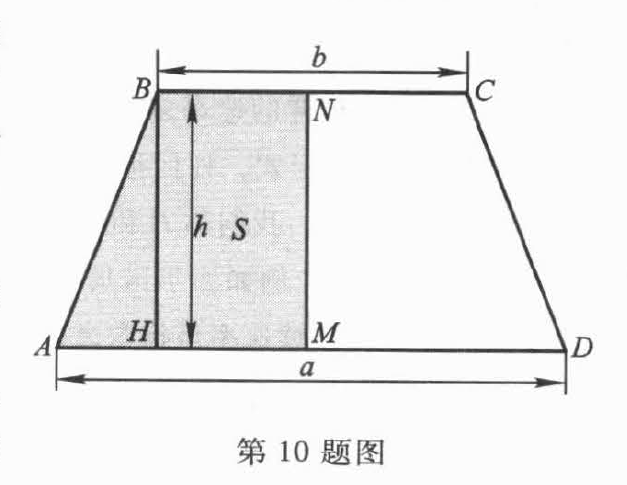
\includegraphics[width=6.5cm,height=5.5cm]{assets/10.png}
%\caption{10题图}
\end{figure}
\end{frame}


\section{练习题}
\subsection{函数}
\begin{frame}{例一}{}
设$f:\mathbb{R} \xrightarrow[]{} \mathbb{R}$严增,$f^{-1}$为其反函数,$x_1$是$f(x)+x=a$的根,$x_2$是$f^{-1}(x)+x=a$的根.试求$x_{1}+x_{2}$的值
\end{frame}
\subsection{函数奇偶性}
\begin{frame}{例二}{}
若$f^{-1}$为$f$的反函数,$y=f^{-1}(-x)$是$y=f(-x)$的反函数,试证$f(x)$为奇函数
\end{frame}
\subsection{周期函数}
\begin{frame}{例三}{}
设$f(x)$是$\mathbb{R}$上的有界实函数,且有
\begin{equation*}
    f(x+h)=\dfrac{f(x+2h)+f(x)}{2} \quad (\forall x \in \mathbb{R})
\end{equation*}
其中$h$为某一确定的正数\\
证明:$h$必是函数$f$的周期
\end{frame}
\end{document}